\justifying

%%----------------------------------------------------
\section{Introduction} \label{sec:intro}
%%----------------------------------------------------

Flares are the largest magnetic event in our solar system. They are characterized by the explosive release of magnetic free energy and localized heating in the solar atmosphere. They manifest differently across various wavelengths. The footpoints of the post flare loops are visible in hard X-ray, for electrons and $\gamma$-rays, for ions. In contrast, the loops are filled with plasma emitting in soft X-ray and Extreme Ultraviolet (EUV) \citep{fletcher11}. The corresponding white light and Near Ultraviolet (NUV) counterparts arise due to changes in ionization and local opacity in the photospheric and chromospheric heights. These are usually some of the most impulsive signatures of flares \citep{watanabe17,hudson06}. The NUV and white light emission have also been demonstrated to be co-spatial and co-temporal with hard X-ray \citep{hudson92, oliverso12}. One of the major puzzling aspects regarding the origin and energetics of solar flares is the origin of the white light (WL) continuum. According to the standard model of flares, the energetic electrons are accelerated along the loops and are stopped via numerous collisions and thermalization when the ambient medium has enough density, usually known as the `thick target' model (For further details, please refer to \cite{brown73,benz17,fletcher11}). We usually believe that these densities are reached within the chromosphere. This explains the co-spatial and co-temporal nature of WL and Hard X-ray. The theory, on the other hand, predicts parts of the WL being created in the upper photosphere, depths inaccessible to electrons in the standard `thick-target' model. 

There have been various attempts to modify the thick target model to account for various observations from solar flares, e.g. a warm target model \cite{kontar15,kontar19}, local re-acceleration of electrons \citep{brown73}, acceleration of protons along with electrons which are expected to penetrate deeper. There were also attempts to explain the source of WL with photospheric `back-warming' \citep{metclaff90}, where the upper photosphere is ionized via energy transported radiatively from the chromosphere. There have been several observations where the WL emission has been associated with enhancement observed in the 2832~{\AA} continuum of IRIS SJI \citep{heinzel14,kleint16,kleint17,kowalski17,kowalski19}. In this paper, we discuss the {\suit} observations of the February 22, 2024, X-class flare. Continuum bright kernels were observed in the red wing (283~nm) and blue wing (276~nm) of the Mg window. To the best of our knowledge, this is the first observation of continuum enhancement of the blue wing of Mg window. The rest of the paper is structured as follows: in \S\ref{sec:obs} we discuss the observations of the flare from various observatories, i.e, {\suit}, IRIS, GOES and STIX. In \S\ref{sec:bright_ker}, we discuss the observations specifically related to the penumbral bright kernels and how they compare across various wavelengths. In \S3, We summarize our findings and discuss the implications it can have regarding our understanding of the origin of WL emission is solar flares.

%%%%%%% ############# %%%%%%%
\section{Observation \& Data Analysis}\label{sec:obs}
%%%%%%% ############# %%%%%%%

NOAA AR 13590 was visible on the north-east of the Solar disk on February 22, 2024. The AR was around a large sunspot in a cluster of sunspots, accompanied by a complex magnetic field structure. The active region flared multiple times during the same day, including an X1.7 flare that peaked around $\sim$ 06:32 UT, an M4.8 flare that peaked around $\sim$ 20:46 UT and an X6.3 flare that peaked $\sim$ 22:34 UT . {\suit} is equipped with an onboard flare detection algorithm. Once the flare detection algorithm flags a flare and localizes the position of the flare on the detector, the program sequence prioritizes reading a fixed smaller Region of Interest (RoI) around the location for fast, higher cadence observation (for further details, please refer to \cite{flare_det}). The X6.3 flare was one of the first flares to be flagged by the on-board flare detection algorithm. {\suit} did not observe the X1.7 flare because, during that time, the payload was off-pointed to verify the stellar calibration program sequences. The flares were also observed by {\it SDO}/AIA, {\it SO}/STIX. {\it IRIS} observed the eastern edge of the X6.3 flare ribbons in a small [66",62"] field of view (FoV) with a 4-step raster and 15 s raster cadence.

%%%%%%%%%%%%%%%%%%%
\begin{figure*}
    \centering
    \includegraphics[trim = {2cm 2.5cm 2.8cm 1.8cm}, clip, width=\linewidth]{Figures/feb_22nd/fig_1.pdf} 
    \caption[SUIT observation of the flare at the respective peak of all filters]{(a) Parts of the full-disk (2k$\times$2k) observation in NB4 (Mg II h) showing the flaring region and sunspot. The dashed magenta box marks the extent of the {\suit} RoI used for the subsequent analysis. {(b)} Cropped observation of the flare from the magenta dashed box in (a), from various science filters of \suit. Two bright umbral kernels are marked in NB2 and NB5 with blue arrows.}
    \label{fig:flare_obs}
\end{figure*}
%%%%%%%%%%%%%%%%%%%

Fig.~\ref{fig:flare_obs}a shows a cutout of the full-disk (2k$\times$2k) observation in NB4 (Mg II h). The magenta dashed box shows the region considered for the subsequent analysis in this paper. We plot the observation from the dashed magenta box marked in Fig.~\ref{fig:flare_obs}a in various \suit~narrow bands during their respective peaks in Fig.~\ref{fig:flare_obs}b. The NB2 (Mg II blue wing), NB3 (Mg II k), NB4 (Mg II h) and NB5 (Mg II red wing) cover the entire Mg window. NB7 and NB8 show the continuum on the red side of the Balmer jump and the Ca II h line, respectively. We see two kernels of umbral brightening during the respective peaks of NB2 and NB5 (marked by white and black arrows in Fig.~\ref{fig:flare_obs}b respectively).

The X6.3 flare provides a good example of the response of the local plasma environment to the flare in the NUV regime in 200 {--} 400 nm. The flare peaked around $\sim$ 22:34 UT in the {\it GOES} observation. Images from six narrow band (NB) channels of {\suit} are shown in Fig.~\ref{fig:flare_obs}c at around $\sim$ 22:28-22:29 UT. This is at the peak of the NB3 (Mg II k 279.6 nm) channel, as observed by \suit. The 60\% peak intensity contour of the NB3 intensity is marked with the black line in all figures of Fig.~\ref{fig:flare_obs}c. From the figure, we also see a similar structure in the NB4 (Mg II h 280.3 nm) and NB8 (Ca II h 396.9 nm). No similar structure is observed in the other continuum channels of Fig.~\ref{fig:flare_obs}c.

%%%%%%%%%
\begin{figure*}
    \centering
    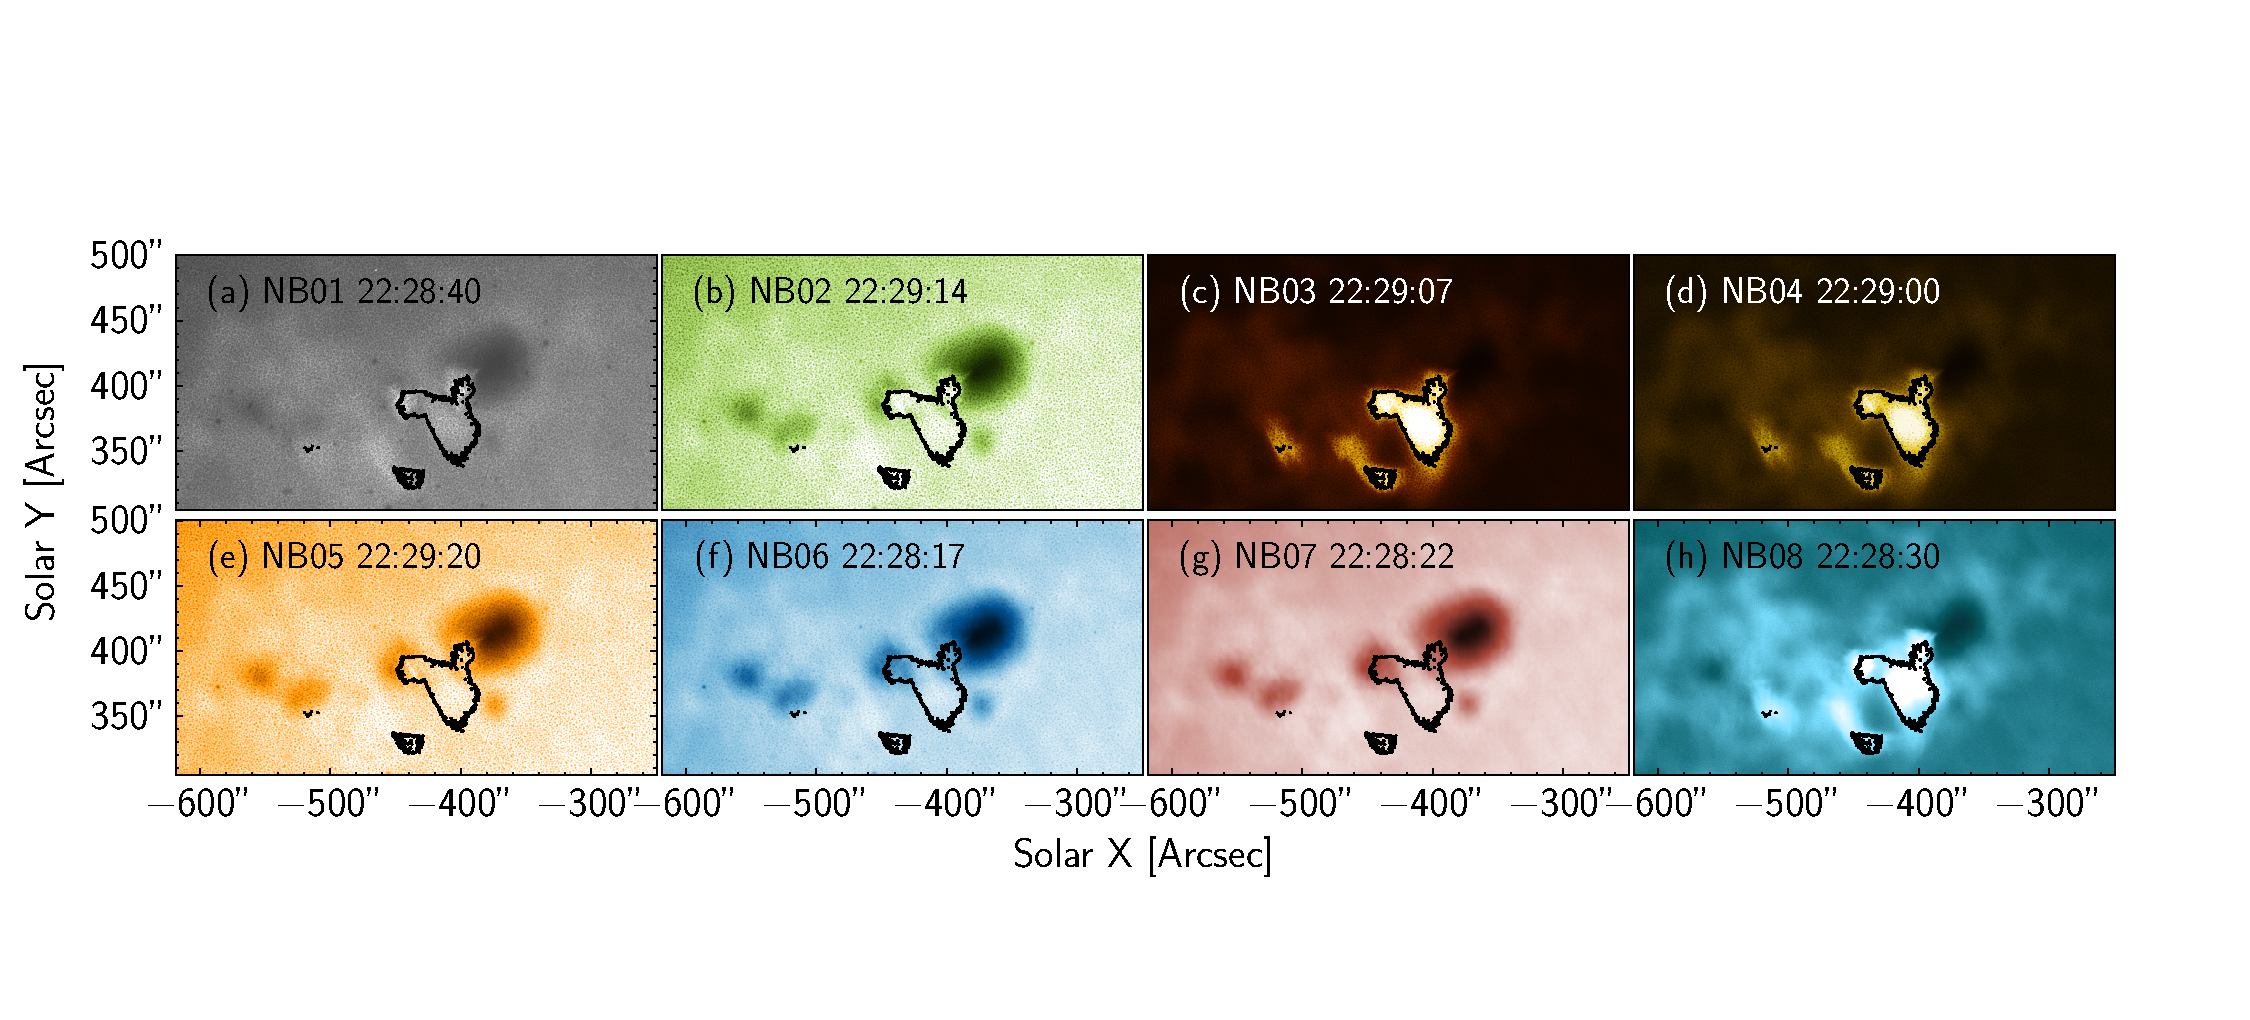
\includegraphics[trim={0.2cm 2.5cm 2cm 4cm},clip,width=\linewidth]{Figures/feb_22nd/suit_roi_nb3_peak.pdf}
    \caption[{\suit} observations of the flare from various NB filters during NB3 peak]{{\suit} observations of the flare from various NB filters during NB3 peak. 60\% peak intensity contour of NB3 is marked across the NB filter observations.}
    \label{fig:flare_nb3_peak}
\end{figure*}
%%%%%%%%%

In Fig.~\ref{fig:flare_lc_suit}.a, we show the GOES 1 {--} 8 {\AA} light curve in comparison to the peak normalised NB3, NB4 and NB8 light curves. All the NB light curves behave remarkably similarly. The vertical dotted black line across all the panels in Fig.~\ref{fig:flare_lc_suit} denotes the peak intensity in NB3. NB3, NB4, and NB8 peaks at the same time around $\sim$ 22:29 UT. We co-align and co-register {\it GONG}-H$\alpha$ observation with SUIT observations and plot the light curve from the same contour region. The {\it GONG} light curve also peaks at around $\sim$ 22:29 UT. Both NB8 and {\it GONG}-H$\alpha$ show less contrast variation in the light curve than NB3 and NB4.

We show the GOES 1 {--} 8 {\AA} light curve in comparison to the NB5 (Redwing of the Mg lines, blue dashed), NB6 and NB7 continuum channels in Fig.~\ref{fig:flare_lc_suit}b. NB5 shows signs of flare response, although much weaker than NB3, NB4 and NB8. NB5 peaks around $\sim$ 22:31 UT, about $\sim$ 3 minutes later than NB3. Similar traits were observed from the images also, as pointed out in Fig.~\ref{fig:flare_obs}c and the accompanying discussions. More interestingly, NB6 (green dot-dashed line) and NB7 (black dotted line) do not show the hallmark sign of a flare light curve, i.e. gradual increase and decrease in the intensity. These bands exhibit a sharp rise in intensity during the impulsive phase of the flare. Finally, in Fig.~\ref{fig:flare_lc_suit}c, we show the {\it GOES} 1 {--} 8 {\AA} light curve in comparison to the STIX hard and soft X-ray light curve. The hard X-ray peaks around a similar time, around $\sim$ 22:29 UT, similar to NB3.

%%%%%%%%%
\begin{figure*}
    \centering
    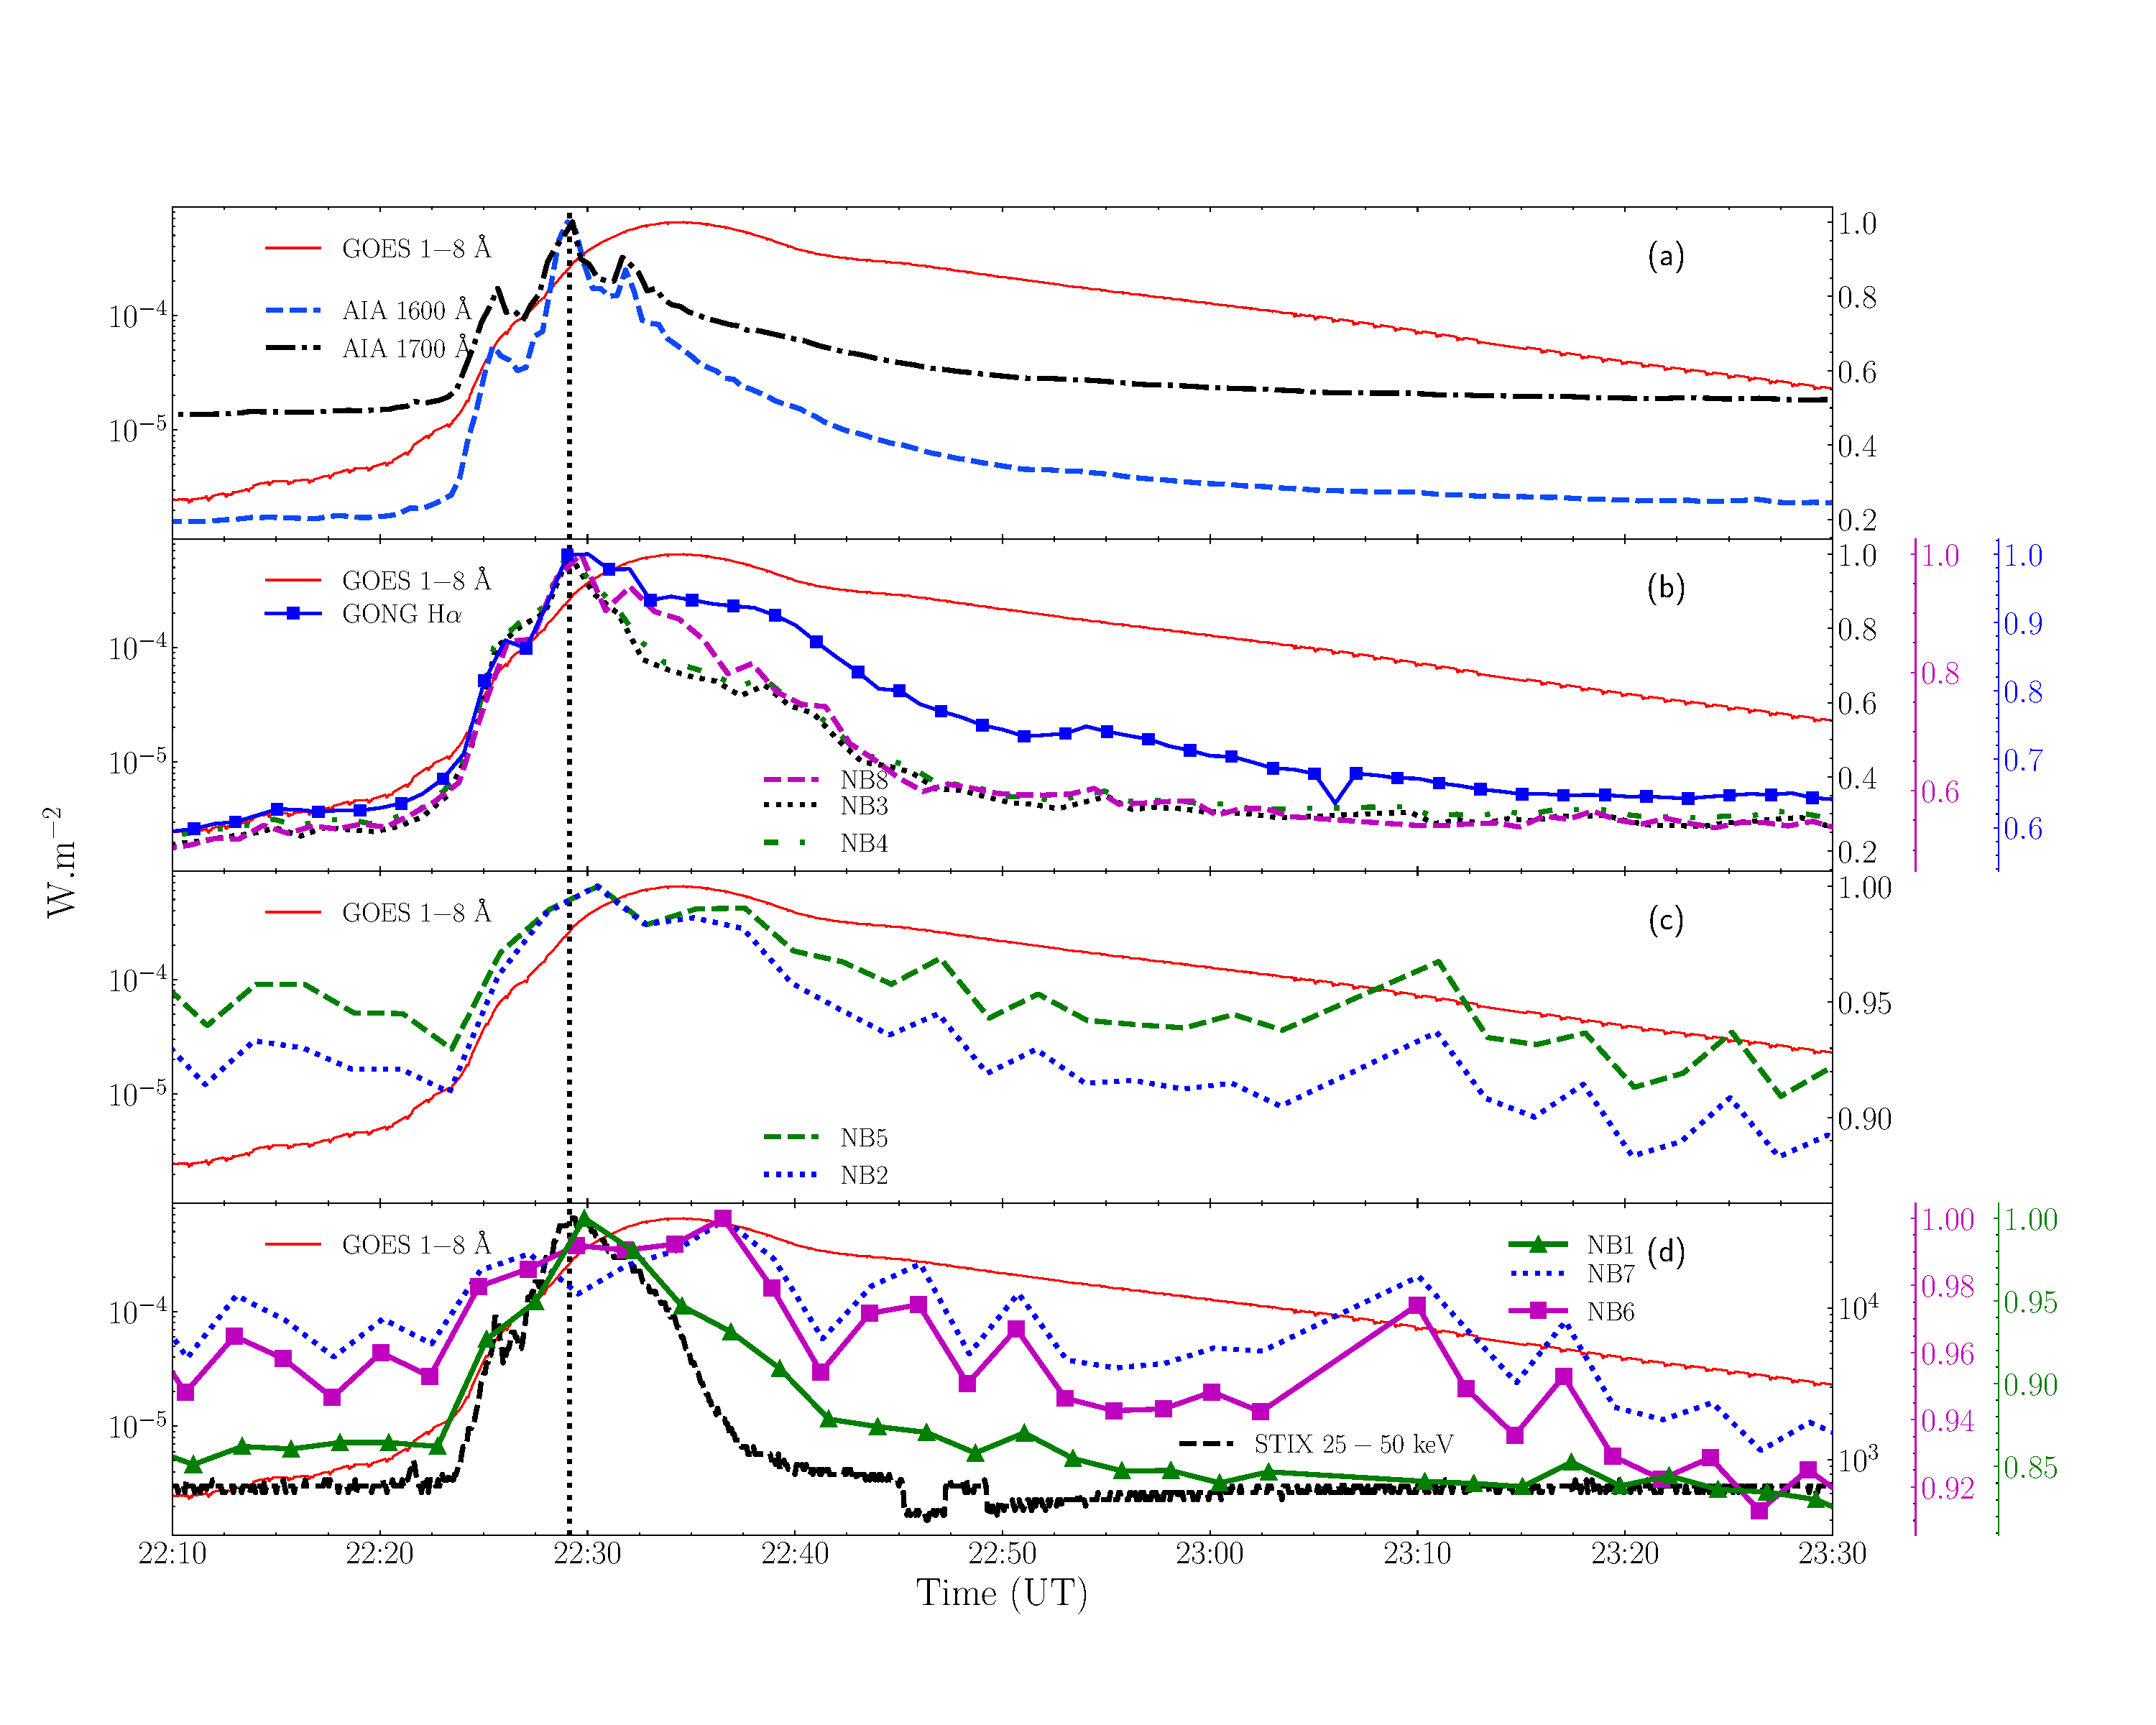
\includegraphics[width=0.9\textwidth,trim={1cm 2cm 1cm 4.2cm},clip]{Figures/feb_22nd/lc_4.pdf}
    \caption[Light curve of the {\suit} NB3 contour from various observatories]{{\bf Top panel:} Light curves from the pixels within intensity contour picked from \suit~NB3, NB4, NB8 and co-aligned GONG H$\alpha$ observations in comparison to the GOES SXR light curve. The NB4 light curve in the first panel is offset by -0.1 s from NB3 for better visibility. The vertical dotted dark line marks the flare's peak in NB3 observation. {\bf Middle panel:} the light curve arising from the NB2 and NB5 pixels from within the NB3 intensity contour in comparison to the GOES SXR light curve. {\bf Bottom panel:} the STIX HXR, NB6, NB7 and NB1 lightcurve compared to the GOES SXR lightcurve. }
    \label{fig:flare_lc_suit}
\end{figure*}
%%%%%%%%%

%%%%%%%%%%%%
\subsubsection{Observation and characterization of the umbral bright kernels}\label{sec:bright_ker}
%%%%%%%%%%%%

One of the curious features of this flare was the short-lived transient bright kernels observed in NB2 and NB5. Similar observations were made by \cite{kowalski19}. They observed umbral brightness kernels in the IRIS SJI 2832 {\AA}~channel for the X1 solar flare SOL2014-10-25T17:08:00. The SJI 2832 {\AA}~probes the sun in a similar wavelength range as {\suit} NB5. They observed the umbral brightening to be arising from a plethora of photospheric absorption lines, mostly Fe II going into emission. They attributed photospheric heating as the cause for the Fe II absorption lines going into emission. Unfortunately, as IRIS was not observing the main flaring region, there is no way to comment on the spectral nature of the brightening kernels. This might indicate the possible observation of new flare lines in the blue wing of the \ion{Mg}{2} lines. We further investigate the light curves of the bright kernels to possibly comment on their origin.

We compare the light curves arising from the bright kernels with GOES soft X-ray and STIX hard X-ray in Fig.~\ref{fig:nb2_lc}. The top panels show the NB2 and NB5 observations at their respective peaks. The two bright kernels are marked with a black dotted line, and a magenta dashed line. The counts from these marked regions are added to create the light curves for the bright kernels. In Fig.~\ref{fig:nb2_lc} middle and bottom panel, we compare the GOES soft X-ray and STIX hard X-ray light curves with respect to the bright kernels observed in NB2 and NB5, respectively. We observed that in NB2, the peak of the light curve is co-temporal with STIX hard X-ray. In NB5, the peak appears slightly later than the hard X-ray peak.  

%%%%%%%%%
\begin{figure*}
    \centering
    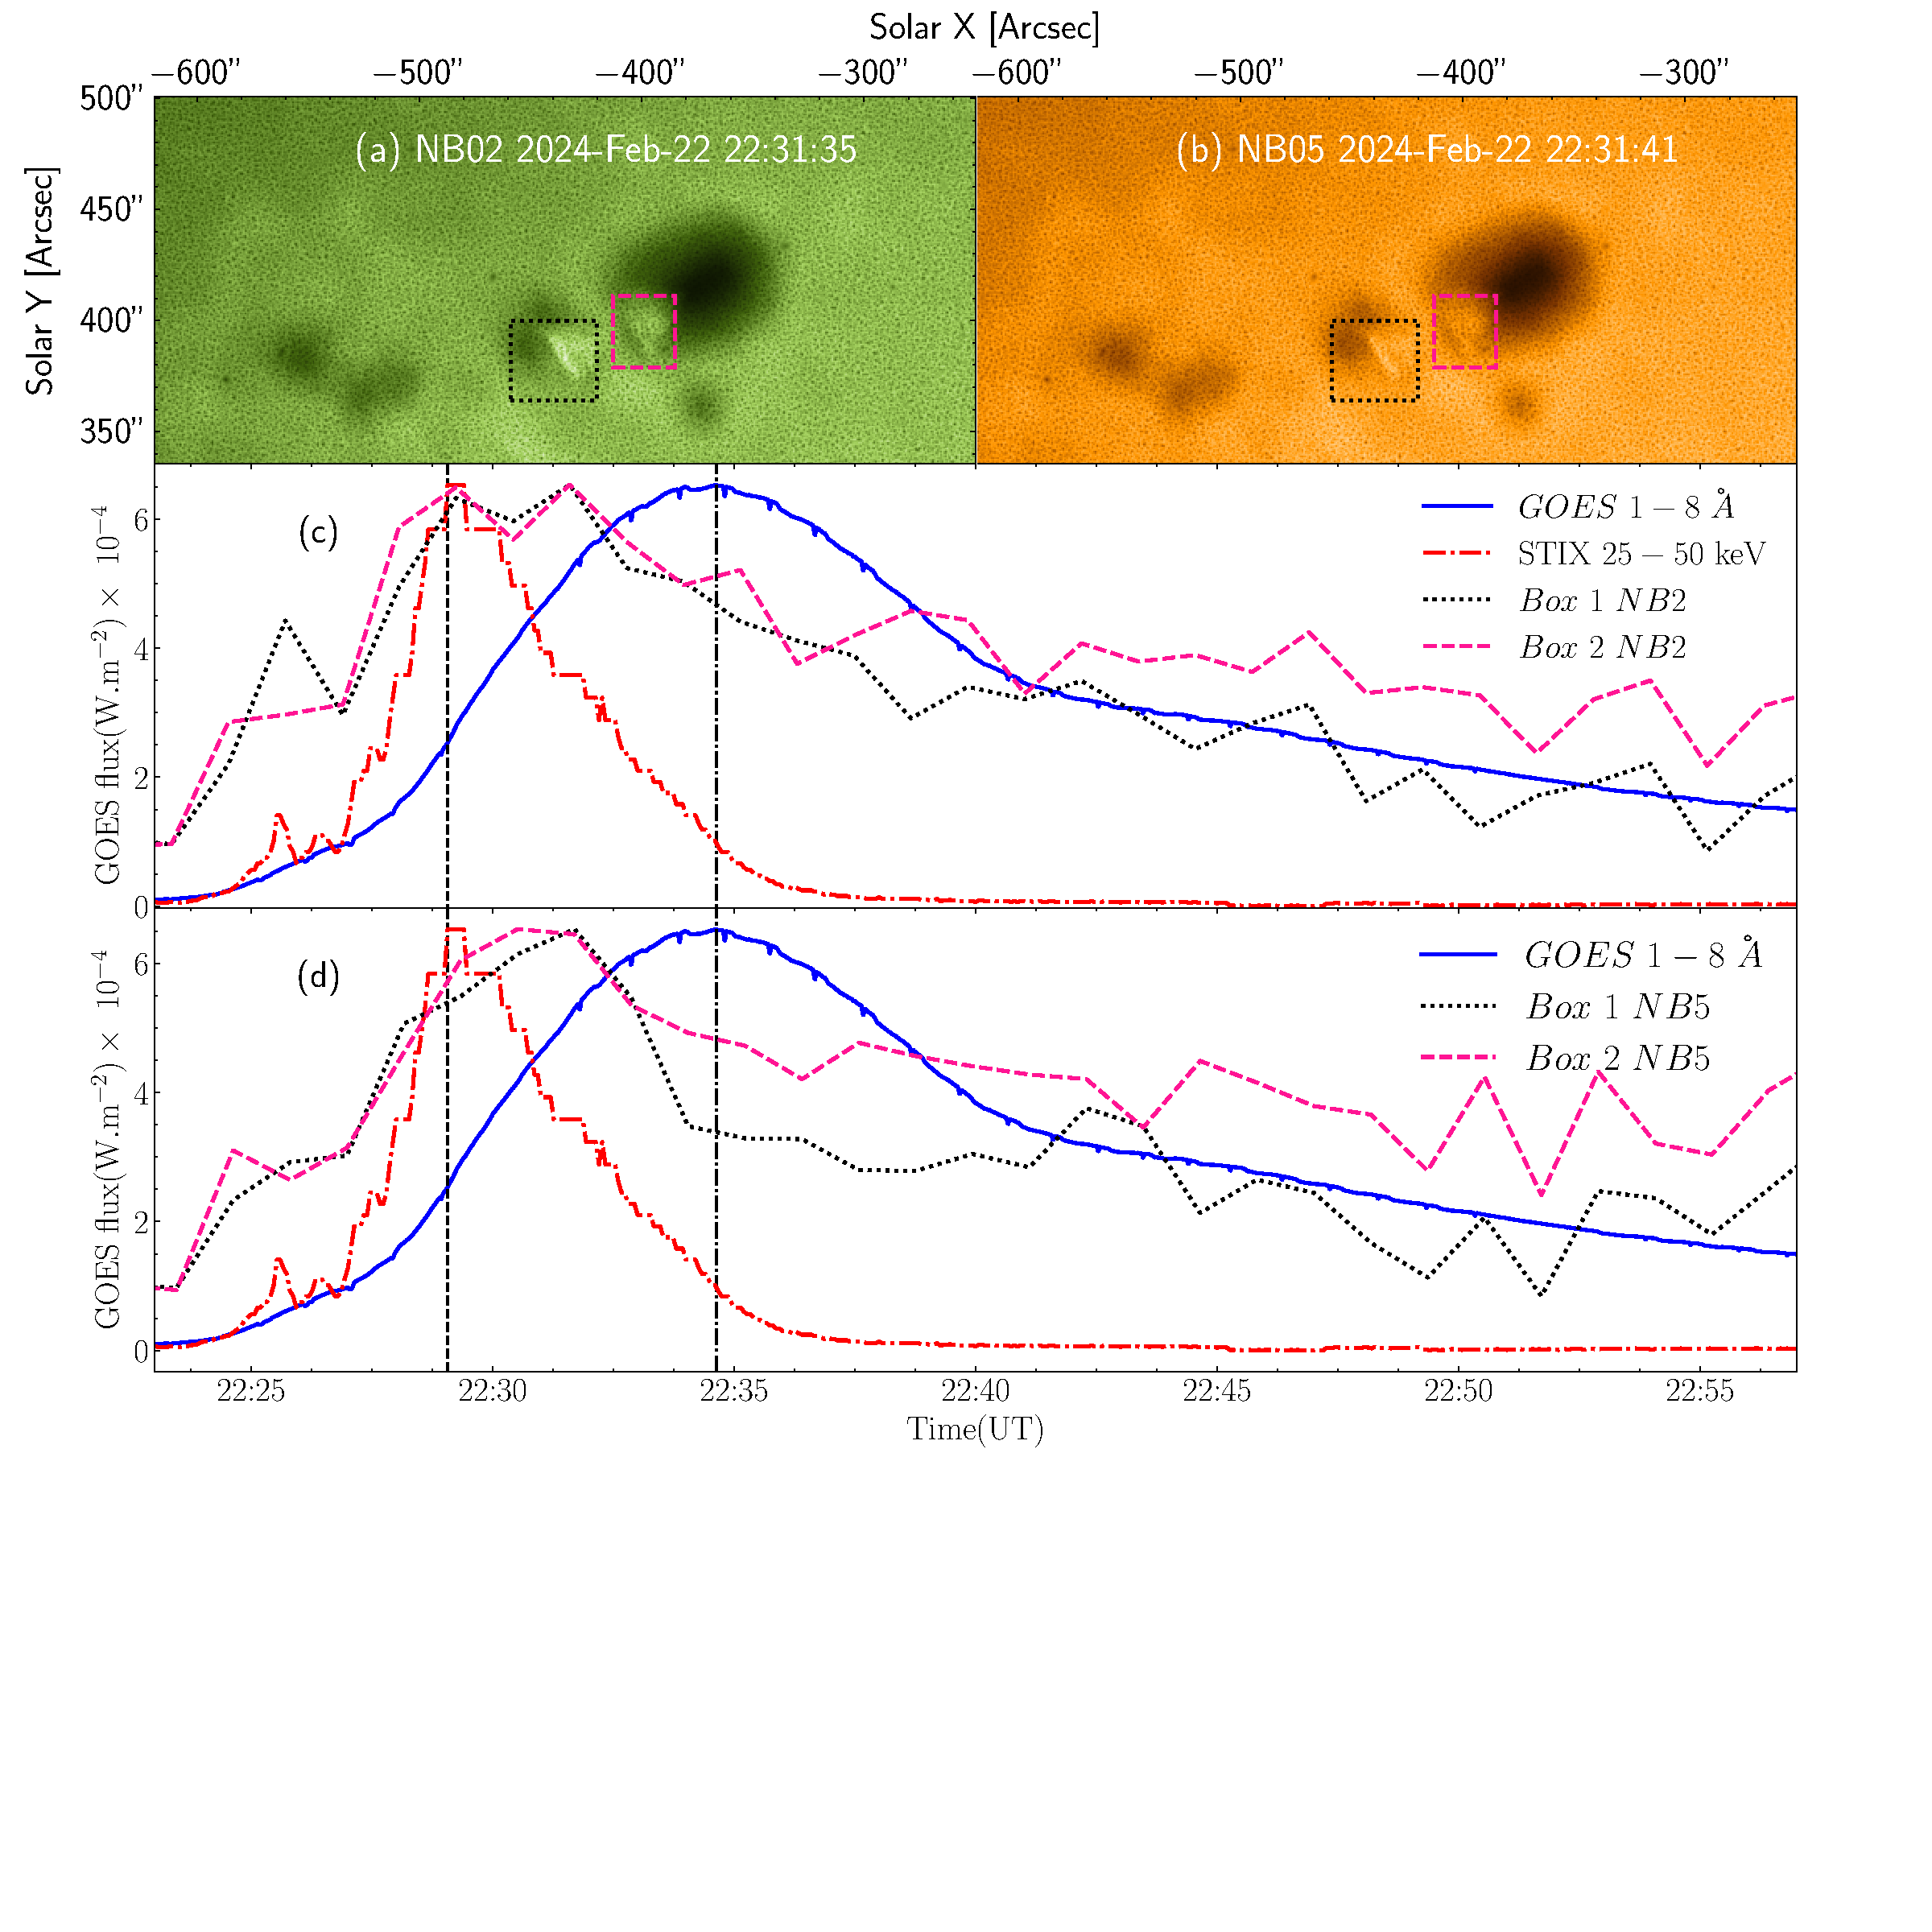
\includegraphics[width=0.9\textwidth,trim={0.5cm 10cm 2cm 0.2cm},clip]{Figures/feb_22nd/nb2_nb5_ker.pdf}
    \caption[Observation of the penumbral bright kernels in NB02 and NB05]{{\bf Top panels}: The NB2 and NB5 observation during the respective peaks. The bright penumbral kernels are marked with black dots and magenta dashed boxes. {\bf Middle panel}: Light curve of the two boxes from NB2 in comparison to GOES 1 {--} 8~{\AA} and STIX 25{--}80 keV light curve. {\bf Bottom panel}: Light curve of the two boxes from NB5 in comparison to GOES 1 {--} 8~{\AA} and STIX 25{--}80 keV light curve. The vertical dashed and dot-dashed lines mark the peaks of STIX hard X-ray and GOES soft X-ray light curves.}
    \label{fig:nb2_lc}
\end{figure*}
%%%%%%%%%

%%%%%%%%%
\subsection{Discussion}\label{sec:disc}
%%%%%%%%%

In this letter, we highlighted the first {\suit} observations of an X-class flare. We see penumbral bright kernels and enhancement in the red wing of the Mg window, similar to \cite{kowalski19,kowalski17,kleint17}. In most cases, these continuum enhancements are associated with WL flares. In this event, we also see bright kernels and enhancements in the blue wing of the Mg window. To the best of our knowledge, this is the first such observation in the blue wing. Unfortunately, we can not comment on the spectral nature of the bright kernels as {\suit} is only an imager. Further exploration is necessary to comment on the spectral nature of the bright kernels.